\documentclass[../document.tex]{subfiles}
\documentclass{beamer}
\usepackage{amssymb,amsmath,amsthm}
\usepackage{graphicx}
\usepackage{tikz}
%\usetheme{Singapore}
\usetheme{Boadilla}
\usecolortheme{rose}

\usetikzlibrary{tikzmark}
\usepackage{colortbl}
\usepackage{graphicx}
\usepackage{pdfpages}
\tikzstyle{every picture}+=[remember picture,baseline]
\tikzstyle{every node}+=[inner sep=0pt,anchor=base,
minimum width=1.5cm,align=center,text depth=.25ex,outer sep=1.5pt]
\tikzstyle{every path}+=[thick, rounded corners]
%\setframetemplate{frametitle}[default][center]

%%%%%%%%%%%%%%%%%%%% VERY IMPORTANT 
%very useful way to add notes to Beamer
%\setbeameroption{show notes on second screen=right}
\setbeamertemplate{note page} 
{ 
	\insertslideintonotes{0.65} 
	\rule{\textwidth}{0.1pt} 
	\color{blue} \small
	\insertnote 
}


% A very important tool to add curly braces for multiple lines, equipping us with \rcases and \lcases. COLOL!!!!!
\usepackage{mathtools}

\begin{document}

\begin{frame}{Signed messages}
	\uncover <1->{\Large What was wrong with the oral messages?\newline}
	\uncover<2->{\normalsize Answer: because \textbf{traitors lie}, they \textbf{alter the contents} of the messages they receive and send. \newline}
	\uncover<3>{\begin{tikzpicture}[remember picture,overlay]
			\node at(current 	page.south) { %for relative positioning, we use \node [left=1cm or right or below or above] 
				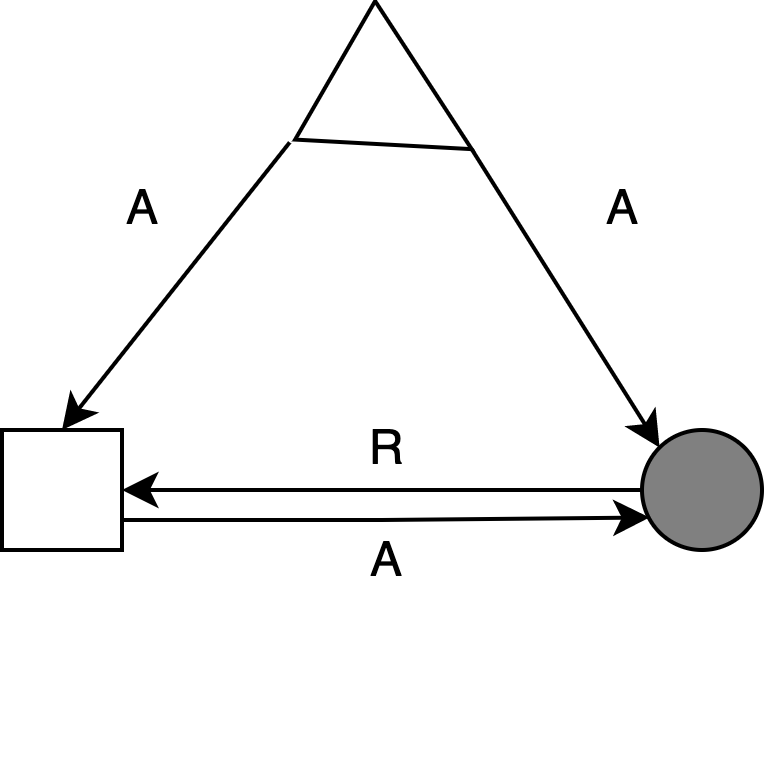
\includegraphics[width=0.4\textwidth]{../fig1.png}	
			};
	\end{tikzpicture}}
	\uncover<4>{Let's make messages that can not be lied (forged) or any alterations could be detected}
\end{frame}


%%%%%%%%%%%%%

\begin{frame}{Formal \textbf{\&abstract} Assumptions regarding Messages!}
$
\begin{rcases}
	\text{A1. Every Message that is sent is delivered correctly.}\\
	\text{A2. There receiver of a message knows who sent it.}\\
	\text{A3. The absence of a message can be detected.}
\end{rcases}\rightarrow \textbf{Oral messages}
$\newline \newline
\large
 \\ A4. (a) A loyal general's signature cannot be forged (\textbf{or changed!!}) and any alteration of the contents of his signed messages can be detected \\
	(b) Anyone can verify the authenticity of a general's signature\newline 
	\centering $\downarrow$
		 \begin{center}
		 	\small \textbf{Signed messages}
		 \end{center}
	BUT, in case of assuming A4, What is the purpose of a traitor?????
\end{frame}

%%%%%%%%%%%%%%


\begin{frame}{Signed messages algorithm}
	\uncover<1>{Note that we know  \textbf{the number of m} traitors when running the Alg.}
	\begin{enumerate}
		\item<2-> Commander sends a \textbf{message} having a value $v$ and a signature (which is a sequence of IDs) $\rightarrow \pmb{v:0}$
		\item<3-> each lieutenant $i$ receives the message of length $k$, \\ \textbf{adds the $v$ to a $V_i$ set}, \textbf{adds his ID} to the message and \textbf{sends it to those child lieutenants not having received this message before}
		\item <4-> when lieutenant $i$ receives no more messages, the lieutenant $i$ applies the \textbf{a Choice function} to $V_i$ in order to retrieve an order.
	\end{enumerate}
	\uncover<5>{What is that \textbf{Choice function?}}	
\end{frame}

%%%%%%%%%%%%%%%%%

\begin{frame}{Choice function}
	\uncover<+-> The Choice function could be any \textbf{aggregate function} (such as median, average, etc) \large BUT, \normalsize it needs to have two essential properties:
	\begin{enumerate}
		\item <+-> if Set $V_i$ consists of single value $v$ Then, $Choice(V_i)={v}$
		\item<+-> $Choice(\emptyset) = RETREAT$ 
	\end{enumerate} 
\end{frame}

%%%%%%%%%%%%%
%%we should use [fragile] for using verbatim environment
\begin{frame}[fragile]{Formal statement of Signed messages $SM(m)$}

	Initially $V_i=\emptyset$\\
	(1) The commander signs and sends message $v:0$ to all lieutenants\\
	(2) For each $i$:\newline 
	\null \quad(A) If Lieutenant $i$ receives a message of the form $v:0$ from the commander and he hasn't receieved any order, then:\\
	\quad \quad(i) he lets $V_i={v}$\\ 
	\quad \quad (ii) he sends the message $v:0:i$ to every other lieutenant.\newline \newline
	\null \quad (B) If Lieutenant $i$ receives a message of the form $v:0:j_1\dots:j_k$ \textbf{and} $v\notin V_i$ then:\\
	\quad \quad(i) he adds $v$ to $V_i$;\\
	\quad \quad (ii) if $k<m$, then he sends the message $v:0:j_1\dots:j_k:i$ to every lieutenant other than $j_1,\dots,j_k$\newline \newline
	(3) For each $i$: When Lieutenant i will receive no more messages, he obeys the order $Choice(V_i)$
\end{frame}

%%%%%%%%%%%%

\begin{frame}{The impossible case revisited}
	\begin{tikzpicture}[remember picture,overlay]
		\node at(current 	page.south) { %for relative positioning, we use \node [left=1cm or right or below or above] 
			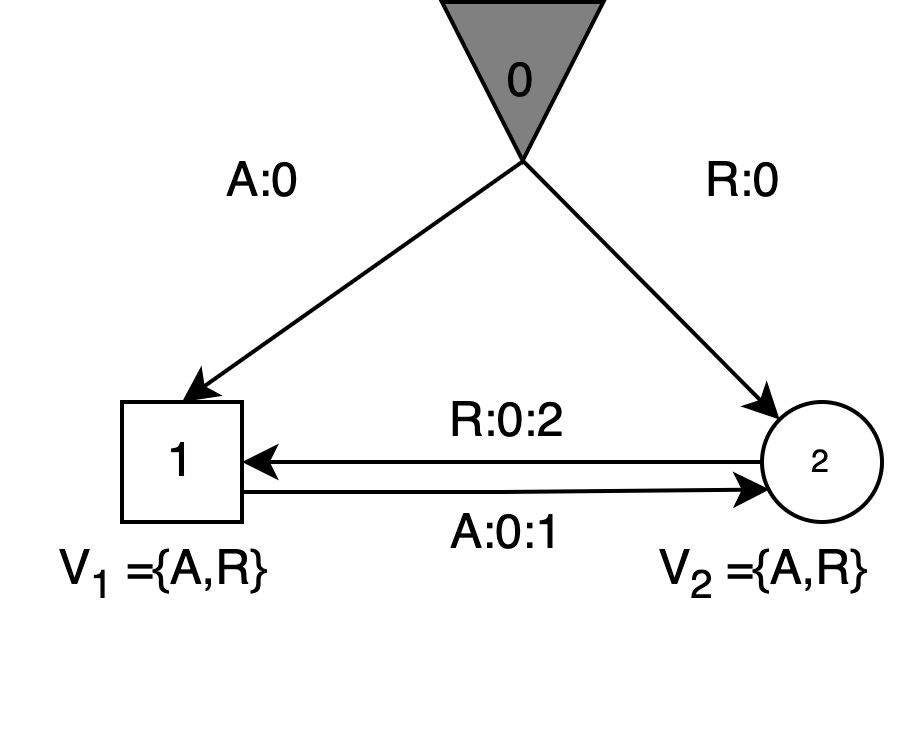
\includegraphics[width=0.8\textwidth]{../fig3.png}	
		};
	\end{tikzpicture}
\end{frame}

%%%%%%%%%%%%%

\begin{frame}
	\begin{itemize}
	\item<+-> The proposed algorithm \textbf{increased fault tolerance}, \\ but it is still \textbf{expensive} $\rightarrow O(n!)$ 
	\item <+-> In what follows, we give a description of a more \textbf{practical and efficient algorithm} which can tolerate Byzantine-faults (i.e. arbitrary messages and faults in nodes) in asynchronous systems, proposed by \textit{Castro M. \& Liskov B.} 
	\item<+-> but first let us define what is meant by \textbf{synchronous and asynchronous systems.}
\end{itemize}
\end{frame}


\end{document}